\documentclass{article}

\usepackage{fancyvrb}
\usepackage [english]{babel}
\usepackage [autostyle, english = american]{csquotes}
\usepackage{graphicx}
\usepackage{hyperref}

\MakeOuterQuote{"}
\graphicspath{ {./assets/FSMs/diagrams/} }

\title{Project \#1 | Lexical Analyzer}
\author{Jared Dyreson, Chris Nutter}
\date{California State University, Fullerton}

\begin{document}
\maketitle
\tableofcontents
\newpage

\section{Introduction}
This project was intended to be a lexical analyzer for our compiler and was aptly named "Lexi".
The goal of Lexi is to parse out the contents of a source document and generate meaningful lexemes.
These lexemes were to adhere to a specific set of regular expressions to define a token.
\section{How to Use}
   \begin{enumerate}
        \item[0.]\textbf{Use a Unix-based OS.}
        \item Extract \textbf{\emph{lexi.zip}}
        \item Enter \emph{lexical\_analysis} folder
        \item Run \textbf{\emph{make}} in Terminal
        \item Output can be run again with \textbf{\emph{./lexi [input]}}
   \end{enumerate}

\section{Design}
    \subsection{Regular Expression}
        The way \emph{Lexi} parses each line and determines the identifier type is through the use of \emph{regular expressions}. Being able to determine the identifier is crucial in defining the token's contents. \emph{Lexi} after processing the file and creating a vector of strings that parses line by line which is then fed through a function that reads each character and determines one of the each lexeme types.

        \begin{enumerate}

            \item \emph{\textbf{Comments}} determines any line that has \emph{!} and ends with a trailing \emph{!}. Multiple comments in a line are supported.
            \begin{Verbatim}
        (!.*!)
            \end{Verbatim}
            
            \item \emph{\textbf{Keywords}} finds any word that is considered reserved for the structure of the language including data types, control-flow operators, and other key-defining words for the language.  
            \begin{Verbatim}
        (int|float|bool|true|false|(end)?if|else|then|while(end)?
        |do(end)?|for(end)?|(in|out)put|and|or|not)
            \end{Verbatim}
            
            \item \emph{\textbf{Number}} is any integer, float, double, size\_t, (etc.) value for identifying amount. 
            \begin{Verbatim}
        (?:\b)([-+]?\d*.?\d+)?(?=\b)
            \end{Verbatim}

            \item \emph{\textbf{Identifier}} grabs any word that is not within a \emph{comment} or \emph{keyword} field.
            \begin{Verbatim}
        ([a-zA-Z]+(\d*)?) 
            \end{Verbatim}
            
            \item \emph{\textbf{Separators}} finds any symbol that helps keep the contents contained.
            \begin{Verbatim}
        ((|)|{|}|[|]|"|'|,)
            \end{Verbatim}
            
            \item \emph{\textbf{Operators}} obtains symbols that the language uses for operation.
            \begin{Verbatim}
        (+|-|*|/|=|>|<|>=|<=|&+||+|%|^!$|^)
            \end{Verbatim}
           
            \item \emph{\textbf{Terminators}} are symbols signalling end of a line.
            \begin{Verbatim}
        (;|$) 
            \end{Verbatim}

        \end{enumerate}


    \subsection{Finite State Machines}
        \begin{figure}[!hbtp]
            \centering
            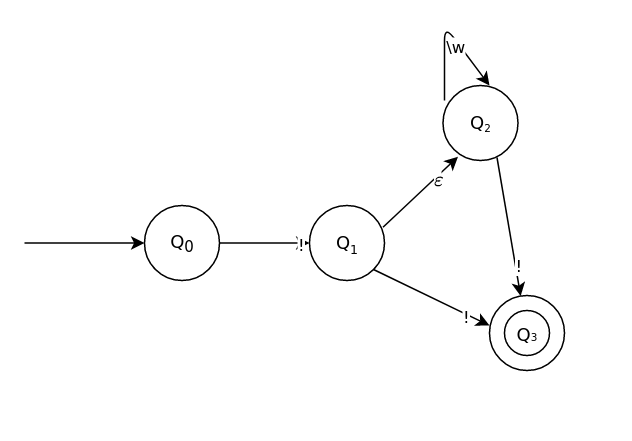
\includegraphics[width=10cm]{Comment-FSM.png}
            \caption{Comment}
        \end{figure}

       \begin{figure}[!hbtp]
            \centering
            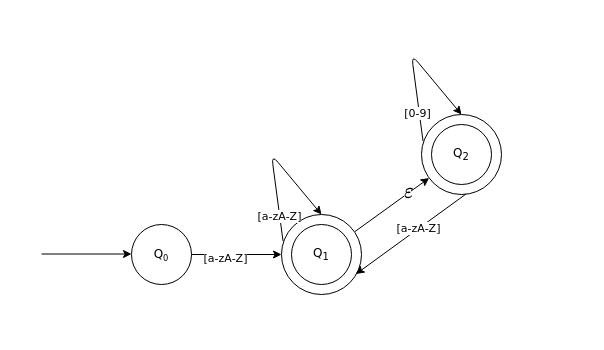
\includegraphics[width=10cm]{Identifier.png}
            \caption{Identifier}
        \end{figure}

       \begin{figure}[!hbtp]
            \centering
            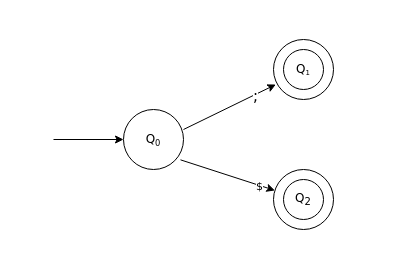
\includegraphics[width=10cm]{Terminators.png}
            \caption{Terminator}
        \end{figure}

\newpage

\section{Shortcomings}
    We had problems generating FSMs for large regular expressions that would be a headache to be written out. 
    Creating formatting for line numbers with comments was a headache due to comments' lengths being fairly large and not being inline.

\end{document}
